\documentclass[twoside]{book}

% Packages required by doxygen
\usepackage{fixltx2e}
\usepackage{calc}
\usepackage{doxygen}
\usepackage[export]{adjustbox} % also loads graphicx
\usepackage{graphicx}
\usepackage[utf8]{inputenc}
\usepackage{makeidx}
\usepackage{multicol}
\usepackage{multirow}
\PassOptionsToPackage{warn}{textcomp}
\usepackage{textcomp}
\usepackage[nointegrals]{wasysym}
\usepackage[table]{xcolor}

% Font selection
\usepackage[T1]{fontenc}
\usepackage[scaled=.90]{helvet}
\usepackage{courier}
\usepackage{amssymb}
\usepackage{sectsty}
\renewcommand{\familydefault}{\sfdefault}
\allsectionsfont{%
  \fontseries{bc}\selectfont%
  \color{darkgray}%
}
\renewcommand{\DoxyLabelFont}{%
  \fontseries{bc}\selectfont%
  \color{darkgray}%
}
\newcommand{\+}{\discretionary{\mbox{\scriptsize$\hookleftarrow$}}{}{}}

% Page & text layout
\usepackage{geometry}
\geometry{%
  a4paper,%
  top=2.5cm,%
  bottom=2.5cm,%
  left=2.5cm,%
  right=2.5cm%
}
\tolerance=750
\hfuzz=15pt
\hbadness=750
\setlength{\emergencystretch}{15pt}
\setlength{\parindent}{0cm}
\setlength{\parskip}{3ex plus 2ex minus 2ex}
\makeatletter
\renewcommand{\paragraph}{%
  \@startsection{paragraph}{4}{0ex}{-1.0ex}{1.0ex}{%
    \normalfont\normalsize\bfseries\SS@parafont%
  }%
}
\renewcommand{\subparagraph}{%
  \@startsection{subparagraph}{5}{0ex}{-1.0ex}{1.0ex}{%
    \normalfont\normalsize\bfseries\SS@subparafont%
  }%
}
\makeatother

% Headers & footers
\usepackage{fancyhdr}
\pagestyle{fancyplain}
\fancyhead[LE]{\fancyplain{}{\bfseries\thepage}}
\fancyhead[CE]{\fancyplain{}{}}
\fancyhead[RE]{\fancyplain{}{\bfseries\leftmark}}
\fancyhead[LO]{\fancyplain{}{\bfseries\rightmark}}
\fancyhead[CO]{\fancyplain{}{}}
\fancyhead[RO]{\fancyplain{}{\bfseries\thepage}}
\fancyfoot[LE]{\fancyplain{}{}}
\fancyfoot[CE]{\fancyplain{}{}}
\fancyfoot[RE]{\fancyplain{}{\bfseries\scriptsize Generated by Doxygen }}
\fancyfoot[LO]{\fancyplain{}{\bfseries\scriptsize Generated by Doxygen }}
\fancyfoot[CO]{\fancyplain{}{}}
\fancyfoot[RO]{\fancyplain{}{}}
\renewcommand{\footrulewidth}{0.4pt}
\renewcommand{\chaptermark}[1]{%
  \markboth{#1}{}%
}
\renewcommand{\sectionmark}[1]{%
  \markright{\thesection\ #1}%
}

% Indices & bibliography
\usepackage{natbib}
\usepackage[titles]{tocloft}
\setcounter{tocdepth}{3}
\setcounter{secnumdepth}{5}
\makeindex

% Hyperlinks (required, but should be loaded last)
\usepackage{ifpdf}
\ifpdf
  \usepackage[pdftex,pagebackref=true]{hyperref}
\else
  \usepackage[ps2pdf,pagebackref=true]{hyperref}
\fi
\hypersetup{%
  colorlinks=true,%
  linkcolor=blue,%
  citecolor=blue,%
  unicode%
}

% Custom commands
\newcommand{\clearemptydoublepage}{%
  \newpage{\pagestyle{empty}\cleardoublepage}%
}

\usepackage{caption}
\captionsetup{labelsep=space,justification=centering,font={bf},singlelinecheck=off,skip=4pt,position=top}

%===== C O N T E N T S =====

\begin{document}

% Titlepage & ToC
\hypersetup{pageanchor=false,
             bookmarksnumbered=true,
             pdfencoding=unicode
            }
\pagenumbering{alph}
\begin{titlepage}
\vspace*{7cm}
\begin{center}%
{\Large Project }\\
\vspace*{1cm}
{\large Generated by Doxygen 1.8.13}\\
\end{center}
\end{titlepage}
\clearemptydoublepage
\pagenumbering{roman}
\tableofcontents
\clearemptydoublepage
\pagenumbering{arabic}
\hypersetup{pageanchor=true}

%--- Begin generated contents ---
\chapter{Hierarchical Index}
\section{Class Hierarchy}
This inheritance list is sorted roughly, but not completely, alphabetically\+:\begin{DoxyCompactList}
\item \contentsline{section}{Audio\+File$<$ T $>$}{\pageref{class_audio_file}}{}
\item \contentsline{section}{Audio\+File$<$ double $>$}{\pageref{class_audio_file}}{}
\item \contentsline{section}{Signal}{\pageref{class_signal}}{}
\item \contentsline{section}{Standard\+Filter$<$ T $>$}{\pageref{class_standard_filter}}{}
\begin{DoxyCompactList}
\item \contentsline{section}{Mean\+Filter$<$ T $>$}{\pageref{class_mean_filter}}{}
\end{DoxyCompactList}
\end{DoxyCompactList}

\chapter{Class Index}
\section{Class List}
Here are the classes, structs, unions and interfaces with brief descriptions\-:\begin{DoxyCompactList}
\item\contentsline{section}{\hyperlink{class_audio_file}{Audio\-File$<$ T $>$} }{\pageref{class_audio_file}}{}
\item\contentsline{section}{\hyperlink{class_signal}{Signal} }{\pageref{class_signal}}{}
\item\contentsline{section}{\hyperlink{class_standard_filter}{Standard\-Filter$<$ T $>$} }{\pageref{class_standard_filter}}{}
\end{DoxyCompactList}

\chapter{File Index}
\section{File List}
Here is a list of all documented files with brief descriptions\-:\begin{DoxyCompactList}
\item\contentsline{section}{\hyperlink{_audio_file_8cpp}{Audio\-File.\-cpp} }{\pageref{_audio_file_8cpp}}{}
\item\contentsline{section}{\hyperlink{_audio_file_8h}{Audio\-File.\-h} }{\pageref{_audio_file_8h}}{}
\item\contentsline{section}{{\bfseries Signal.\-h} }{\pageref{_signal_8h}}{}
\item\contentsline{section}{{\bfseries Standard\-Filter.\-h} }{\pageref{_standard_filter_8h}}{}
\end{DoxyCompactList}

\chapter{Class Documentation}
\hypertarget{class_audio_file}{}\section{Audio\+File$<$ T $>$ Class Template Reference}
\label{class_audio_file}\index{Audio\+File$<$ T $>$@{Audio\+File$<$ T $>$}}
\subsection*{Public Types}
\begin{DoxyCompactItemize}
\item 
\mbox{\Hypertarget{class_audio_file_ad1260a47791dc30cbabfe3ff2ea099b1}\label{class_audio_file_ad1260a47791dc30cbabfe3ff2ea099b1}} 
typedef std\+::vector$<$ std\+::vector$<$ T $>$ $>$ {\bfseries Audio\+Buffer}
\end{DoxyCompactItemize}
\subsection*{Public Member Functions}
\begin{DoxyCompactItemize}
\item 
\hyperlink{class_audio_file_ae74399e93d3f4623c7421ee10cfc0e15}{Audio\+File} ()
\item 
bool \hyperlink{class_audio_file_a0ff16123b519a4665e9f3e7d341f0a26}{load} (std\+::string file\+Path)
\item 
bool \hyperlink{class_audio_file_a415239cad5b54b4fef4a210ab79911e3}{save} (std\+::string file\+Path, \hyperlink{_audio_file_8h_ad18559d169602e85d0ad68da6ef8593f}{Audio\+File\+Format} format=Audio\+File\+Format\+::\+Wave)
\item 
uint32\+\_\+t \hyperlink{class_audio_file_a8cd1b082af9db6bd180e4a63edcdefc9}{get\+Sample\+Rate} () const
\item 
int \hyperlink{class_audio_file_a514f860a956b4494ee8d8c806391d6b3}{get\+Num\+Channels} () const
\item 
bool \hyperlink{class_audio_file_a1057326fd2c2eca7cc7937f811868cf1}{is\+Mono} () const
\item 
bool \hyperlink{class_audio_file_a380a188d95f8f23b7622dfe222a7e8f6}{is\+Stereo} () const
\item 
int \hyperlink{class_audio_file_a5495d5cb55911de54f0714e219130b48}{get\+Bit\+Depth} () const
\item 
int \hyperlink{class_audio_file_ae1b5b4b7351a79dbf810bb34ede496b9}{get\+Num\+Samples\+Per\+Channel} () const
\item 
double \hyperlink{class_audio_file_a5a6b01404675361b1c21c9c5fb5753d4}{get\+Length\+In\+Seconds} () const
\item 
void \hyperlink{class_audio_file_a7b88c68133a9ac92149c58499e026360}{print\+Summary} () const
\item 
bool \hyperlink{class_audio_file_afa0a0f7d576b0597c938c5a89746636e}{set\+Audio\+Buffer} (Audio\+Buffer \&new\+Buffer)
\item 
void \hyperlink{class_audio_file_ac155ed12db0f3b02011a7d75b525e71a}{set\+Audio\+Buffer\+Size} (int num\+Channels, int num\+Samples)
\item 
void \hyperlink{class_audio_file_a4cff9513d49e21d25de13513564784b7}{set\+Num\+Samples\+Per\+Channel} (int num\+Samples)
\item 
void \hyperlink{class_audio_file_a354018a94ae15907d7308782f2adadbb}{set\+Num\+Channels} (int num\+Channels)
\item 
void \hyperlink{class_audio_file_a2adf2ea23e7daeb8401e717c1b3d874b}{set\+Bit\+Depth} (int num\+Bits\+Per\+Sample)
\item 
void \hyperlink{class_audio_file_a2d8fa306e40535113c3eba111e16483b}{set\+Sample\+Rate} (uint32\+\_\+t new\+Sample\+Rate)
\end{DoxyCompactItemize}
\subsection*{Public Attributes}
\begin{DoxyCompactItemize}
\item 
Audio\+Buffer \hyperlink{class_audio_file_af937119db095c5af870851050dcbeabb}{samples}
\end{DoxyCompactItemize}
\subsection*{Protected Types}
\begin{DoxyCompactItemize}
\item 
\mbox{\Hypertarget{class_audio_file_a4d5f3a950f0c059380d268abf39fd67e}\label{class_audio_file_a4d5f3a950f0c059380d268abf39fd67e}} 
enum {\bfseries Endianness} \{ {\bfseries Little\+Endian}, 
{\bfseries Big\+Endian}
 \}
\end{DoxyCompactItemize}
\subsection*{Protected Member Functions}
\begin{DoxyCompactItemize}
\item 
\mbox{\Hypertarget{class_audio_file_a0d55bc7ae7b9eb014b93b6baabab8ba7}\label{class_audio_file_a0d55bc7ae7b9eb014b93b6baabab8ba7}} 
\hyperlink{_audio_file_8h_ad18559d169602e85d0ad68da6ef8593f}{Audio\+File\+Format} {\bfseries determine\+Audio\+File\+Format} (std\+::vector$<$ uint8\+\_\+t $>$ \&file\+Data)
\item 
\mbox{\Hypertarget{class_audio_file_afea0b1dbe7788155f249fa3b8a0ad693}\label{class_audio_file_afea0b1dbe7788155f249fa3b8a0ad693}} 
bool {\bfseries decode\+Wave\+File} (std\+::vector$<$ uint8\+\_\+t $>$ \&file\+Data)
\item 
\mbox{\Hypertarget{class_audio_file_a1d68d689475374b830c3e41d7cd54dfa}\label{class_audio_file_a1d68d689475374b830c3e41d7cd54dfa}} 
bool {\bfseries decode\+Aiff\+File} (std\+::vector$<$ uint8\+\_\+t $>$ \&file\+Data)
\item 
\mbox{\Hypertarget{class_audio_file_a9b1997f2466ec1674ce17bebb9a1ba2d}\label{class_audio_file_a9b1997f2466ec1674ce17bebb9a1ba2d}} 
bool {\bfseries save\+To\+Wave\+File} (std\+::string file\+Path)
\item 
\mbox{\Hypertarget{class_audio_file_aa6ed89cc0884105f7022c7595c1609ea}\label{class_audio_file_aa6ed89cc0884105f7022c7595c1609ea}} 
bool {\bfseries save\+To\+Aiff\+File} (std\+::string file\+Path)
\item 
\mbox{\Hypertarget{class_audio_file_a4859348770aba2ab8638a6d2d29490ad}\label{class_audio_file_a4859348770aba2ab8638a6d2d29490ad}} 
void {\bfseries clear\+Audio\+Buffer} ()
\item 
\mbox{\Hypertarget{class_audio_file_a5fcde4e965721804e6f60fc38936887f}\label{class_audio_file_a5fcde4e965721804e6f60fc38936887f}} 
int32\+\_\+t {\bfseries four\+Bytes\+To\+Int} (std\+::vector$<$ uint8\+\_\+t $>$ \&source, int start\+Index, Endianness endianness=Endianness\+::\+Little\+Endian)
\item 
\mbox{\Hypertarget{class_audio_file_a279bb7ae95e4b3b9db5e9c9e141b564d}\label{class_audio_file_a279bb7ae95e4b3b9db5e9c9e141b564d}} 
int16\+\_\+t {\bfseries two\+Bytes\+To\+Int} (std\+::vector$<$ uint8\+\_\+t $>$ \&source, int start\+Index, Endianness endianness=Endianness\+::\+Little\+Endian)
\item 
\mbox{\Hypertarget{class_audio_file_a7446935a450d4aa8da37e5ac1fd4133b}\label{class_audio_file_a7446935a450d4aa8da37e5ac1fd4133b}} 
int {\bfseries get\+Index\+Of\+String} (std\+::vector$<$ uint8\+\_\+t $>$ \&source, std\+::string s)
\item 
\mbox{\Hypertarget{class_audio_file_a2ff18ea40f28f1758f0ca78b2185c789}\label{class_audio_file_a2ff18ea40f28f1758f0ca78b2185c789}} 
T {\bfseries sixteen\+Bit\+Int\+To\+Sample} (int16\+\_\+t sample)
\item 
\mbox{\Hypertarget{class_audio_file_afd351555e7868d1c9cbf77d93edc09dd}\label{class_audio_file_afd351555e7868d1c9cbf77d93edc09dd}} 
uint32\+\_\+t {\bfseries get\+Aiff\+Sample\+Rate} (std\+::vector$<$ uint8\+\_\+t $>$ \&file\+Data, int sample\+Rate\+Start\+Index)
\item 
\mbox{\Hypertarget{class_audio_file_a801f2c42d590c1fcba274c6d1f70cfbc}\label{class_audio_file_a801f2c42d590c1fcba274c6d1f70cfbc}} 
bool {\bfseries ten\+Byte\+Match} (std\+::vector$<$ uint8\+\_\+t $>$ \&v1, int start\+Index1, std\+::vector$<$ uint8\+\_\+t $>$ \&v2, int start\+Index2)
\item 
\mbox{\Hypertarget{class_audio_file_aa25ff369a0e2ca315c7abf3982ef1c18}\label{class_audio_file_aa25ff369a0e2ca315c7abf3982ef1c18}} 
void {\bfseries add\+Sample\+Rate\+To\+Aiff\+Data} (std\+::vector$<$ uint8\+\_\+t $>$ \&file\+Data, uint32\+\_\+t sample\+Rate)
\item 
\mbox{\Hypertarget{class_audio_file_a21b500e75c67e28f38554c2eb752e24b}\label{class_audio_file_a21b500e75c67e28f38554c2eb752e24b}} 
void {\bfseries add\+String\+To\+File\+Data} (std\+::vector$<$ uint8\+\_\+t $>$ \&file\+Data, std\+::string s)
\item 
\mbox{\Hypertarget{class_audio_file_add8628d661b806fbba0e28231da97563}\label{class_audio_file_add8628d661b806fbba0e28231da97563}} 
void {\bfseries add\+Int32\+To\+File\+Data} (std\+::vector$<$ uint8\+\_\+t $>$ \&file\+Data, int32\+\_\+t i, Endianness endianness=Endianness\+::\+Little\+Endian)
\item 
\mbox{\Hypertarget{class_audio_file_aba8b98835fdc51bc9d0e04634c70603a}\label{class_audio_file_aba8b98835fdc51bc9d0e04634c70603a}} 
void {\bfseries add\+Int16\+To\+File\+Data} (std\+::vector$<$ uint8\+\_\+t $>$ \&file\+Data, int16\+\_\+t i, Endianness endianness=Endianness\+::\+Little\+Endian)
\item 
\mbox{\Hypertarget{class_audio_file_a734c540c871a3843f01f908bbfc3962d}\label{class_audio_file_a734c540c871a3843f01f908bbfc3962d}} 
bool {\bfseries write\+Data\+To\+File} (std\+::vector$<$ uint8\+\_\+t $>$ \&file\+Data, std\+::string file\+Path)
\end{DoxyCompactItemize}
\subsection*{Protected Attributes}
\begin{DoxyCompactItemize}
\item 
\mbox{\Hypertarget{class_audio_file_aeafbb547cc9b08418212c41215c57838}\label{class_audio_file_aeafbb547cc9b08418212c41215c57838}} 
\hyperlink{_audio_file_8h_ad18559d169602e85d0ad68da6ef8593f}{Audio\+File\+Format} {\bfseries audio\+File\+Format}
\item 
\mbox{\Hypertarget{class_audio_file_aa8517ad3c63493253ecf59bb0c9974c1}\label{class_audio_file_aa8517ad3c63493253ecf59bb0c9974c1}} 
uint32\+\_\+t {\bfseries sample\+Rate}
\item 
\mbox{\Hypertarget{class_audio_file_a19f9bc02bc118b7c2fa3d50e7bbb49b3}\label{class_audio_file_a19f9bc02bc118b7c2fa3d50e7bbb49b3}} 
int {\bfseries bit\+Depth}
\end{DoxyCompactItemize}


\subsection{Constructor \& Destructor Documentation}
\mbox{\Hypertarget{class_audio_file_ae74399e93d3f4623c7421ee10cfc0e15}\label{class_audio_file_ae74399e93d3f4623c7421ee10cfc0e15}} 
\index{Audio\+File@{Audio\+File}!Audio\+File@{Audio\+File}}
\index{Audio\+File@{Audio\+File}!Audio\+File@{Audio\+File}}
\subsubsection{\texorpdfstring{Audio\+File()}{AudioFile()}}
{\footnotesize\ttfamily template$<$class T $>$ \\
\hyperlink{class_audio_file}{Audio\+File}$<$ T $>$\+::\hyperlink{class_audio_file}{Audio\+File} (\begin{DoxyParamCaption}{ }\end{DoxyParamCaption})}

Constructor 

\subsection{Member Function Documentation}
\mbox{\Hypertarget{class_audio_file_a5495d5cb55911de54f0714e219130b48}\label{class_audio_file_a5495d5cb55911de54f0714e219130b48}} 
\index{Audio\+File@{Audio\+File}!get\+Bit\+Depth@{get\+Bit\+Depth}}
\index{get\+Bit\+Depth@{get\+Bit\+Depth}!Audio\+File@{Audio\+File}}
\subsubsection{\texorpdfstring{get\+Bit\+Depth()}{getBitDepth()}}
{\footnotesize\ttfamily template$<$class T $>$ \\
int \hyperlink{class_audio_file}{Audio\+File}$<$ T $>$\+::get\+Bit\+Depth (\begin{DoxyParamCaption}{ }\end{DoxyParamCaption}) const}

the bit depth of each sample \mbox{\Hypertarget{class_audio_file_a5a6b01404675361b1c21c9c5fb5753d4}\label{class_audio_file_a5a6b01404675361b1c21c9c5fb5753d4}} 
\index{Audio\+File@{Audio\+File}!get\+Length\+In\+Seconds@{get\+Length\+In\+Seconds}}
\index{get\+Length\+In\+Seconds@{get\+Length\+In\+Seconds}!Audio\+File@{Audio\+File}}
\subsubsection{\texorpdfstring{get\+Length\+In\+Seconds()}{getLengthInSeconds()}}
{\footnotesize\ttfamily template$<$class T $>$ \\
double \hyperlink{class_audio_file}{Audio\+File}$<$ T $>$\+::get\+Length\+In\+Seconds (\begin{DoxyParamCaption}{ }\end{DoxyParamCaption}) const}

the length in seconds of the audio file based on the number of samples and sample rate \mbox{\Hypertarget{class_audio_file_a514f860a956b4494ee8d8c806391d6b3}\label{class_audio_file_a514f860a956b4494ee8d8c806391d6b3}} 
\index{Audio\+File@{Audio\+File}!get\+Num\+Channels@{get\+Num\+Channels}}
\index{get\+Num\+Channels@{get\+Num\+Channels}!Audio\+File@{Audio\+File}}
\subsubsection{\texorpdfstring{get\+Num\+Channels()}{getNumChannels()}}
{\footnotesize\ttfamily template$<$class T $>$ \\
int \hyperlink{class_audio_file}{Audio\+File}$<$ T $>$\+::get\+Num\+Channels (\begin{DoxyParamCaption}{ }\end{DoxyParamCaption}) const}

the number of audio channels in the buffer \mbox{\Hypertarget{class_audio_file_ae1b5b4b7351a79dbf810bb34ede496b9}\label{class_audio_file_ae1b5b4b7351a79dbf810bb34ede496b9}} 
\index{Audio\+File@{Audio\+File}!get\+Num\+Samples\+Per\+Channel@{get\+Num\+Samples\+Per\+Channel}}
\index{get\+Num\+Samples\+Per\+Channel@{get\+Num\+Samples\+Per\+Channel}!Audio\+File@{Audio\+File}}
\subsubsection{\texorpdfstring{get\+Num\+Samples\+Per\+Channel()}{getNumSamplesPerChannel()}}
{\footnotesize\ttfamily template$<$class T $>$ \\
int \hyperlink{class_audio_file}{Audio\+File}$<$ T $>$\+::get\+Num\+Samples\+Per\+Channel (\begin{DoxyParamCaption}{ }\end{DoxyParamCaption}) const}

the number of samples per channel \mbox{\Hypertarget{class_audio_file_a8cd1b082af9db6bd180e4a63edcdefc9}\label{class_audio_file_a8cd1b082af9db6bd180e4a63edcdefc9}} 
\index{Audio\+File@{Audio\+File}!get\+Sample\+Rate@{get\+Sample\+Rate}}
\index{get\+Sample\+Rate@{get\+Sample\+Rate}!Audio\+File@{Audio\+File}}
\subsubsection{\texorpdfstring{get\+Sample\+Rate()}{getSampleRate()}}
{\footnotesize\ttfamily template$<$class T $>$ \\
uint32\+\_\+t \hyperlink{class_audio_file}{Audio\+File}$<$ T $>$\+::get\+Sample\+Rate (\begin{DoxyParamCaption}{ }\end{DoxyParamCaption}) const}

the sample rate \mbox{\Hypertarget{class_audio_file_a1057326fd2c2eca7cc7937f811868cf1}\label{class_audio_file_a1057326fd2c2eca7cc7937f811868cf1}} 
\index{Audio\+File@{Audio\+File}!is\+Mono@{is\+Mono}}
\index{is\+Mono@{is\+Mono}!Audio\+File@{Audio\+File}}
\subsubsection{\texorpdfstring{is\+Mono()}{isMono()}}
{\footnotesize\ttfamily template$<$class T $>$ \\
bool \hyperlink{class_audio_file}{Audio\+File}$<$ T $>$\+::is\+Mono (\begin{DoxyParamCaption}{ }\end{DoxyParamCaption}) const}

true if the audio file is mono \mbox{\Hypertarget{class_audio_file_a380a188d95f8f23b7622dfe222a7e8f6}\label{class_audio_file_a380a188d95f8f23b7622dfe222a7e8f6}} 
\index{Audio\+File@{Audio\+File}!is\+Stereo@{is\+Stereo}}
\index{is\+Stereo@{is\+Stereo}!Audio\+File@{Audio\+File}}
\subsubsection{\texorpdfstring{is\+Stereo()}{isStereo()}}
{\footnotesize\ttfamily template$<$class T $>$ \\
bool \hyperlink{class_audio_file}{Audio\+File}$<$ T $>$\+::is\+Stereo (\begin{DoxyParamCaption}{ }\end{DoxyParamCaption}) const}

true if the audio file is stereo \mbox{\Hypertarget{class_audio_file_a0ff16123b519a4665e9f3e7d341f0a26}\label{class_audio_file_a0ff16123b519a4665e9f3e7d341f0a26}} 
\index{Audio\+File@{Audio\+File}!load@{load}}
\index{load@{load}!Audio\+File@{Audio\+File}}
\subsubsection{\texorpdfstring{load()}{load()}}
{\footnotesize\ttfamily template$<$class T $>$ \\
bool \hyperlink{class_audio_file}{Audio\+File}$<$ T $>$\+::load (\begin{DoxyParamCaption}\item[{std\+::string}]{file\+Path }\end{DoxyParamCaption})}

Loads an audio file from a given file path.  true if the file was successfully loaded \mbox{\Hypertarget{class_audio_file_a7b88c68133a9ac92149c58499e026360}\label{class_audio_file_a7b88c68133a9ac92149c58499e026360}} 
\index{Audio\+File@{Audio\+File}!print\+Summary@{print\+Summary}}
\index{print\+Summary@{print\+Summary}!Audio\+File@{Audio\+File}}
\subsubsection{\texorpdfstring{print\+Summary()}{printSummary()}}
{\footnotesize\ttfamily template$<$class T $>$ \\
void \hyperlink{class_audio_file}{Audio\+File}$<$ T $>$\+::print\+Summary (\begin{DoxyParamCaption}{ }\end{DoxyParamCaption}) const}

Prints a summary of the audio file to the console \mbox{\Hypertarget{class_audio_file_a415239cad5b54b4fef4a210ab79911e3}\label{class_audio_file_a415239cad5b54b4fef4a210ab79911e3}} 
\index{Audio\+File@{Audio\+File}!save@{save}}
\index{save@{save}!Audio\+File@{Audio\+File}}
\subsubsection{\texorpdfstring{save()}{save()}}
{\footnotesize\ttfamily template$<$class T $>$ \\
bool \hyperlink{class_audio_file}{Audio\+File}$<$ T $>$\+::save (\begin{DoxyParamCaption}\item[{std\+::string}]{file\+Path,  }\item[{\hyperlink{_audio_file_8h_ad18559d169602e85d0ad68da6ef8593f}{Audio\+File\+Format}}]{format = {\ttfamily AudioFileFormat\+:\+:Wave} }\end{DoxyParamCaption})}

Saves an audio file to a given file path.  true if the file was successfully saved \mbox{\Hypertarget{class_audio_file_afa0a0f7d576b0597c938c5a89746636e}\label{class_audio_file_afa0a0f7d576b0597c938c5a89746636e}} 
\index{Audio\+File@{Audio\+File}!set\+Audio\+Buffer@{set\+Audio\+Buffer}}
\index{set\+Audio\+Buffer@{set\+Audio\+Buffer}!Audio\+File@{Audio\+File}}
\subsubsection{\texorpdfstring{set\+Audio\+Buffer()}{setAudioBuffer()}}
{\footnotesize\ttfamily template$<$class T $>$ \\
bool \hyperlink{class_audio_file}{Audio\+File}$<$ T $>$\+::set\+Audio\+Buffer (\begin{DoxyParamCaption}\item[{Audio\+Buffer \&}]{new\+Buffer }\end{DoxyParamCaption})}

Set the audio buffer for this \hyperlink{class_audio_file}{Audio\+File} by copying samples from another buffer.  true if the buffer was copied successfully. \mbox{\Hypertarget{class_audio_file_ac155ed12db0f3b02011a7d75b525e71a}\label{class_audio_file_ac155ed12db0f3b02011a7d75b525e71a}} 
\index{Audio\+File@{Audio\+File}!set\+Audio\+Buffer\+Size@{set\+Audio\+Buffer\+Size}}
\index{set\+Audio\+Buffer\+Size@{set\+Audio\+Buffer\+Size}!Audio\+File@{Audio\+File}}
\subsubsection{\texorpdfstring{set\+Audio\+Buffer\+Size()}{setAudioBufferSize()}}
{\footnotesize\ttfamily template$<$class T $>$ \\
void \hyperlink{class_audio_file}{Audio\+File}$<$ T $>$\+::set\+Audio\+Buffer\+Size (\begin{DoxyParamCaption}\item[{int}]{num\+Channels,  }\item[{int}]{num\+Samples }\end{DoxyParamCaption})}

Sets the audio buffer to a given number of channels and number of samples per channel. This will try to preserve the existing audio, adding zeros to any new channels or new samples in a given channel. \mbox{\Hypertarget{class_audio_file_a2adf2ea23e7daeb8401e717c1b3d874b}\label{class_audio_file_a2adf2ea23e7daeb8401e717c1b3d874b}} 
\index{Audio\+File@{Audio\+File}!set\+Bit\+Depth@{set\+Bit\+Depth}}
\index{set\+Bit\+Depth@{set\+Bit\+Depth}!Audio\+File@{Audio\+File}}
\subsubsection{\texorpdfstring{set\+Bit\+Depth()}{setBitDepth()}}
{\footnotesize\ttfamily template$<$class T $>$ \\
void \hyperlink{class_audio_file}{Audio\+File}$<$ T $>$\+::set\+Bit\+Depth (\begin{DoxyParamCaption}\item[{int}]{num\+Bits\+Per\+Sample }\end{DoxyParamCaption})}

Sets the bit depth for the audio file. If you use the \hyperlink{class_audio_file_a415239cad5b54b4fef4a210ab79911e3}{save()} function, this bit depth rate will be used \mbox{\Hypertarget{class_audio_file_a354018a94ae15907d7308782f2adadbb}\label{class_audio_file_a354018a94ae15907d7308782f2adadbb}} 
\index{Audio\+File@{Audio\+File}!set\+Num\+Channels@{set\+Num\+Channels}}
\index{set\+Num\+Channels@{set\+Num\+Channels}!Audio\+File@{Audio\+File}}
\subsubsection{\texorpdfstring{set\+Num\+Channels()}{setNumChannels()}}
{\footnotesize\ttfamily template$<$class T $>$ \\
void \hyperlink{class_audio_file}{Audio\+File}$<$ T $>$\+::set\+Num\+Channels (\begin{DoxyParamCaption}\item[{int}]{num\+Channels }\end{DoxyParamCaption})}

Sets the number of channels. New channels will have the correct number of samples and be initialised to zero \mbox{\Hypertarget{class_audio_file_a4cff9513d49e21d25de13513564784b7}\label{class_audio_file_a4cff9513d49e21d25de13513564784b7}} 
\index{Audio\+File@{Audio\+File}!set\+Num\+Samples\+Per\+Channel@{set\+Num\+Samples\+Per\+Channel}}
\index{set\+Num\+Samples\+Per\+Channel@{set\+Num\+Samples\+Per\+Channel}!Audio\+File@{Audio\+File}}
\subsubsection{\texorpdfstring{set\+Num\+Samples\+Per\+Channel()}{setNumSamplesPerChannel()}}
{\footnotesize\ttfamily template$<$class T $>$ \\
void \hyperlink{class_audio_file}{Audio\+File}$<$ T $>$\+::set\+Num\+Samples\+Per\+Channel (\begin{DoxyParamCaption}\item[{int}]{num\+Samples }\end{DoxyParamCaption})}

Sets the number of samples per channel in the audio buffer. This will try to preserve the existing audio, adding zeros to new samples in a given channel if the number of samples is increased. \mbox{\Hypertarget{class_audio_file_a2d8fa306e40535113c3eba111e16483b}\label{class_audio_file_a2d8fa306e40535113c3eba111e16483b}} 
\index{Audio\+File@{Audio\+File}!set\+Sample\+Rate@{set\+Sample\+Rate}}
\index{set\+Sample\+Rate@{set\+Sample\+Rate}!Audio\+File@{Audio\+File}}
\subsubsection{\texorpdfstring{set\+Sample\+Rate()}{setSampleRate()}}
{\footnotesize\ttfamily template$<$class T $>$ \\
void \hyperlink{class_audio_file}{Audio\+File}$<$ T $>$\+::set\+Sample\+Rate (\begin{DoxyParamCaption}\item[{uint32\+\_\+t}]{new\+Sample\+Rate }\end{DoxyParamCaption})}

Sets the sample rate for the audio file. If you use the \hyperlink{class_audio_file_a415239cad5b54b4fef4a210ab79911e3}{save()} function, this sample rate will be used 

\subsection{Member Data Documentation}
\mbox{\Hypertarget{class_audio_file_af937119db095c5af870851050dcbeabb}\label{class_audio_file_af937119db095c5af870851050dcbeabb}} 
\index{Audio\+File@{Audio\+File}!samples@{samples}}
\index{samples@{samples}!Audio\+File@{Audio\+File}}
\subsubsection{\texorpdfstring{samples}{samples}}
{\footnotesize\ttfamily template$<$class T$>$ \\
Audio\+Buffer \hyperlink{class_audio_file}{Audio\+File}$<$ T $>$\+::samples}

A vector of vectors holding the audio samples for the \hyperlink{class_audio_file}{Audio\+File}. You can access the samples by channel and then by sample index, i.\+e\+: \begin{DoxyVerb} samples[channel][sampleIndex]\end{DoxyVerb}
 

The documentation for this class was generated from the following files\+:\begin{DoxyCompactItemize}
\item 
\hyperlink{_audio_file_8h}{Audio\+File.\+h}\item 
\hyperlink{_audio_file_8cpp}{Audio\+File.\+cpp}\end{DoxyCompactItemize}

\hypertarget{class_mean_filter}{}\section{Mean\+Filter$<$ T $>$ Class Template Reference}
\label{class_mean_filter}\index{Mean\+Filter$<$ T $>$@{Mean\+Filter$<$ T $>$}}


Inheritance diagram for Mean\+Filter$<$ T $>$\+:\nopagebreak
\begin{figure}[H]
\begin{center}
\leavevmode
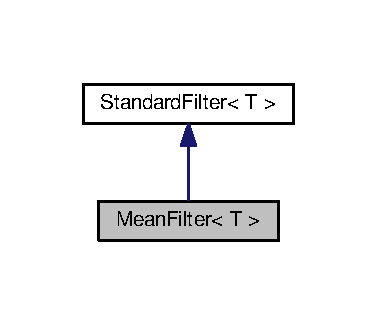
\includegraphics[width=181pt]{class_mean_filter__inherit__graph}
\end{center}
\end{figure}


Collaboration diagram for Mean\+Filter$<$ T $>$\+:\nopagebreak
\begin{figure}[H]
\begin{center}
\leavevmode
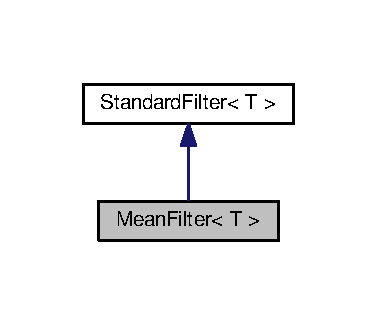
\includegraphics[width=181pt]{class_mean_filter__coll__graph}
\end{center}
\end{figure}
\subsection*{Public Member Functions}
\begin{DoxyCompactItemize}
\item 
\hyperlink{class_mean_filter_a413efd370b9feb8bb7bef736c83356ec}{Mean\+Filter} ()
\item 
\hyperlink{class_mean_filter_a6266059422f16d94fbd2661cb05ffade}{Mean\+Filter} (int p\+Length)
\end{DoxyCompactItemize}
\subsection*{Additional Inherited Members}


\subsection{Constructor \& Destructor Documentation}
\mbox{\Hypertarget{class_mean_filter_a413efd370b9feb8bb7bef736c83356ec}\label{class_mean_filter_a413efd370b9feb8bb7bef736c83356ec}} 
\index{Mean\+Filter@{Mean\+Filter}!Mean\+Filter@{Mean\+Filter}}
\index{Mean\+Filter@{Mean\+Filter}!Mean\+Filter@{Mean\+Filter}}
\subsubsection{\texorpdfstring{Mean\+Filter()}{MeanFilter()}\hspace{0.1cm}{\footnotesize\ttfamily [1/2]}}
{\footnotesize\ttfamily template$<$typename T $>$ \\
\hyperlink{class_mean_filter}{Mean\+Filter}$<$ T $>$\+::\hyperlink{class_mean_filter}{Mean\+Filter} (\begin{DoxyParamCaption}{ }\end{DoxyParamCaption})}

Standard Constructor The length is set to 5 We construct an array of given length with all the entries set as 1/length \mbox{\Hypertarget{class_mean_filter_a6266059422f16d94fbd2661cb05ffade}\label{class_mean_filter_a6266059422f16d94fbd2661cb05ffade}} 
\index{Mean\+Filter@{Mean\+Filter}!Mean\+Filter@{Mean\+Filter}}
\index{Mean\+Filter@{Mean\+Filter}!Mean\+Filter@{Mean\+Filter}}
\subsubsection{\texorpdfstring{Mean\+Filter()}{MeanFilter()}\hspace{0.1cm}{\footnotesize\ttfamily [2/2]}}
{\footnotesize\ttfamily template$<$typename T $>$ \\
\hyperlink{class_mean_filter}{Mean\+Filter}$<$ T $>$\+::\hyperlink{class_mean_filter}{Mean\+Filter} (\begin{DoxyParamCaption}\item[{int}]{p\+Length }\end{DoxyParamCaption})}

Constructor with the length of the mask We construct an array of given length with all the entries set as 1/length 
\begin{DoxyParams}{Parameters}
{\em p\+Length} & int which indicated the length of the filter \\
\hline
\end{DoxyParams}


The documentation for this class was generated from the following files\+:\begin{DoxyCompactItemize}
\item 
Mean\+Filter.\+h\item 
Mean\+Filter\+\_\+imp.\+h\end{DoxyCompactItemize}

\hypertarget{class_signal}{}\section{Signal Class Reference}
\label{class_signal}\index{Signal@{Signal}}
\subsection*{Public Member Functions}
\begin{DoxyCompactItemize}
\item 
\hyperlink{class_signal_adc5d70461299de8a723f2aa59767b13f}{Signal} (std\+::string name)
\item 
\hyperlink{class_signal_ae7a1d116cda63e790bf9aab549d57d3a}{$\sim$\+Signal} ()
\item 
std\+::vector$<$ double $>$ \hyperlink{class_signal_a9e55e5bdd1606e4e21edfd19e31a83df}{get\+Time} () const
\item 
\mbox{\Hypertarget{class_signal_a35b36f112a3bd2593a50c827b9ac1e06}\label{class_signal_a35b36f112a3bd2593a50c827b9ac1e06}} 
\hyperlink{class_audio_file}{Audio\+File}$<$ double $>$ {\bfseries get\+Audio\+File} () const
\end{DoxyCompactItemize}


\subsection{Constructor \& Destructor Documentation}
\mbox{\Hypertarget{class_signal_adc5d70461299de8a723f2aa59767b13f}\label{class_signal_adc5d70461299de8a723f2aa59767b13f}} 
\index{Signal@{Signal}!Signal@{Signal}}
\index{Signal@{Signal}!Signal@{Signal}}
\subsubsection{\texorpdfstring{Signal()}{Signal()}}
{\footnotesize\ttfamily Signal\+::\+Signal (\begin{DoxyParamCaption}\item[{std\+::string}]{name }\end{DoxyParamCaption})}

Constructors \mbox{\Hypertarget{class_signal_ae7a1d116cda63e790bf9aab549d57d3a}\label{class_signal_ae7a1d116cda63e790bf9aab549d57d3a}} 
\index{Signal@{Signal}!````~Signal@{$\sim$\+Signal}}
\index{````~Signal@{$\sim$\+Signal}!Signal@{Signal}}
\subsubsection{\texorpdfstring{$\sim$\+Signal()}{~Signal()}}
{\footnotesize\ttfamily Signal\+::$\sim$\+Signal (\begin{DoxyParamCaption}{ }\end{DoxyParamCaption})}

Destructor 

\subsection{Member Function Documentation}
\mbox{\Hypertarget{class_signal_a9e55e5bdd1606e4e21edfd19e31a83df}\label{class_signal_a9e55e5bdd1606e4e21edfd19e31a83df}} 
\index{Signal@{Signal}!get\+Time@{get\+Time}}
\index{get\+Time@{get\+Time}!Signal@{Signal}}
\subsubsection{\texorpdfstring{get\+Time()}{getTime()}}
{\footnotesize\ttfamily std\+::vector$<$ double $>$ Signal\+::get\+Time (\begin{DoxyParamCaption}{ }\end{DoxyParamCaption}) const}

Getters 

The documentation for this class was generated from the following files\+:\begin{DoxyCompactItemize}
\item 
Signal.\+h\item 
Signal.\+cpp\end{DoxyCompactItemize}

\hypertarget{class_standard_filter}{}\section{Standard\+Filter$<$ T $>$ Class Template Reference}
\label{class_standard_filter}\index{Standard\+Filter$<$ T $>$@{Standard\+Filter$<$ T $>$}}


Inheritance diagram for Standard\+Filter$<$ T $>$\+:\nopagebreak
\begin{figure}[H]
\begin{center}
\leavevmode
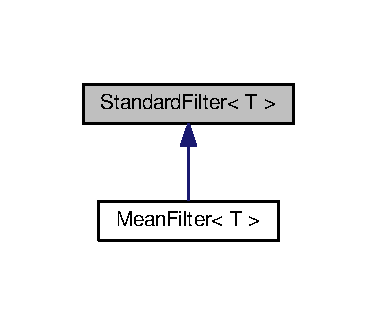
\includegraphics[width=181pt]{class_standard_filter__inherit__graph}
\end{center}
\end{figure}
\subsection*{Public Member Functions}
\begin{DoxyCompactItemize}
\item 
\hyperlink{class_standard_filter_a7ccdce74856a1bdfa877bcec14b5c98b}{Standard\+Filter} ()
\item 
\hyperlink{class_standard_filter_acbc237007e90073c4306e748d73d7eaf}{Standard\+Filter} (int p\+Length)
\item 
\hyperlink{class_standard_filter_a380828493a181b61010bb633538b0e7c}{Standard\+Filter} (std\+::vector$<$ T $>$ p\+Mask)
\item 
\hyperlink{class_standard_filter_a748eb93b291c9f50496015f3c07069a0}{$\sim$\+Standard\+Filter} ()
\item 
void \hyperlink{class_standard_filter_abef27f90eea94d34607e24dd026a281e}{set\+Mask} (std\+::vector$<$ T $>$ p\+Mask)
\item 
std\+::vector$<$ T $>$ \hyperlink{class_standard_filter_ab511fb0167d038d75cba52dd936eddd3}{get\+Mask} ()
\item 
void \hyperlink{class_standard_filter_af441d21022cd441f08421de8cd714d53}{set\+Length} (int p\+Length)
\item 
int \hyperlink{class_standard_filter_ae993492384d41dc26c5f5577607b3b02}{get\+Length} ()
\item 
std\+::vector$<$ T $>$ \hyperlink{class_standard_filter_a2b6a11ed970216b26bda63857d4ed1fc}{apply} (std\+::vector$<$ T $>$ p\+Signal)
\end{DoxyCompactItemize}
\subsection*{Protected Attributes}
\begin{DoxyCompactItemize}
\item 
std\+::vector$<$ T $>$ \hyperlink{class_standard_filter_afc83cf6d1aa9cf9a1ae4a8c476d8a66d}{mask}
\item 
int \hyperlink{class_standard_filter_aa693971cea1c7c485a19928fd77a91c7}{length}
\end{DoxyCompactItemize}


\subsection{Constructor \& Destructor Documentation}
\mbox{\Hypertarget{class_standard_filter_a7ccdce74856a1bdfa877bcec14b5c98b}\label{class_standard_filter_a7ccdce74856a1bdfa877bcec14b5c98b}} 
\index{Standard\+Filter@{Standard\+Filter}!Standard\+Filter@{Standard\+Filter}}
\index{Standard\+Filter@{Standard\+Filter}!Standard\+Filter@{Standard\+Filter}}
\subsubsection{\texorpdfstring{Standard\+Filter()}{StandardFilter()}\hspace{0.1cm}{\footnotesize\ttfamily [1/3]}}
{\footnotesize\ttfamily template$<$typename T $>$ \\
\hyperlink{class_standard_filter}{Standard\+Filter}$<$ T $>$\+::\hyperlink{class_standard_filter}{Standard\+Filter} (\begin{DoxyParamCaption}{ }\end{DoxyParamCaption})}

Standard Constructor The length is set to 5 \mbox{\Hypertarget{class_standard_filter_acbc237007e90073c4306e748d73d7eaf}\label{class_standard_filter_acbc237007e90073c4306e748d73d7eaf}} 
\index{Standard\+Filter@{Standard\+Filter}!Standard\+Filter@{Standard\+Filter}}
\index{Standard\+Filter@{Standard\+Filter}!Standard\+Filter@{Standard\+Filter}}
\subsubsection{\texorpdfstring{Standard\+Filter()}{StandardFilter()}\hspace{0.1cm}{\footnotesize\ttfamily [2/3]}}
{\footnotesize\ttfamily template$<$typename T $>$ \\
\hyperlink{class_standard_filter}{Standard\+Filter}$<$ T $>$\+::\hyperlink{class_standard_filter}{Standard\+Filter} (\begin{DoxyParamCaption}\item[{int}]{p\+Length }\end{DoxyParamCaption})}

Constructor with the length of the mask 
\begin{DoxyParams}{Parameters}
{\em p\+Length} & int which indicated the length of the filter \\
\hline
\end{DoxyParams}
\mbox{\Hypertarget{class_standard_filter_a380828493a181b61010bb633538b0e7c}\label{class_standard_filter_a380828493a181b61010bb633538b0e7c}} 
\index{Standard\+Filter@{Standard\+Filter}!Standard\+Filter@{Standard\+Filter}}
\index{Standard\+Filter@{Standard\+Filter}!Standard\+Filter@{Standard\+Filter}}
\subsubsection{\texorpdfstring{Standard\+Filter()}{StandardFilter()}\hspace{0.1cm}{\footnotesize\ttfamily [3/3]}}
{\footnotesize\ttfamily template$<$typename T $>$ \\
\hyperlink{class_standard_filter}{Standard\+Filter}$<$ T $>$\+::\hyperlink{class_standard_filter}{Standard\+Filter} (\begin{DoxyParamCaption}\item[{std\+::vector$<$ T $>$}]{p\+Mask }\end{DoxyParamCaption})}

Constructor with the mask 
\begin{DoxyParams}{Parameters}
{\em p\+Mask} & std\+::vector$<$\+T$>$ which defines the filter \\
\hline
\end{DoxyParams}
\mbox{\Hypertarget{class_standard_filter_a748eb93b291c9f50496015f3c07069a0}\label{class_standard_filter_a748eb93b291c9f50496015f3c07069a0}} 
\index{Standard\+Filter@{Standard\+Filter}!````~Standard\+Filter@{$\sim$\+Standard\+Filter}}
\index{````~Standard\+Filter@{$\sim$\+Standard\+Filter}!Standard\+Filter@{Standard\+Filter}}
\subsubsection{\texorpdfstring{$\sim$\+Standard\+Filter()}{~StandardFilter()}}
{\footnotesize\ttfamily template$<$typename T $>$ \\
\hyperlink{class_standard_filter}{Standard\+Filter}$<$ T $>$\+::$\sim$\hyperlink{class_standard_filter}{Standard\+Filter} (\begin{DoxyParamCaption}{ }\end{DoxyParamCaption})}

Destructor 

\subsection{Member Function Documentation}
\mbox{\Hypertarget{class_standard_filter_a2b6a11ed970216b26bda63857d4ed1fc}\label{class_standard_filter_a2b6a11ed970216b26bda63857d4ed1fc}} 
\index{Standard\+Filter@{Standard\+Filter}!apply@{apply}}
\index{apply@{apply}!Standard\+Filter@{Standard\+Filter}}
\subsubsection{\texorpdfstring{apply()}{apply()}}
{\footnotesize\ttfamily template$<$typename T $>$ \\
std\+::vector$<$ T $>$ \hyperlink{class_standard_filter}{Standard\+Filter}$<$ T $>$\+::apply (\begin{DoxyParamCaption}\item[{std\+::vector$<$ T $>$}]{p\+Signal }\end{DoxyParamCaption})}

Applies the filter to the signal 
\begin{DoxyParams}{Parameters}
{\em \hyperlink{class_signal}{Signal}} & the signal to which we want to apply the filter. \\
\hline
\end{DoxyParams}
\begin{DoxyReturn}{Returns}
the \hyperlink{class_signal}{Signal} filtered 
\end{DoxyReturn}
\mbox{\Hypertarget{class_standard_filter_ae993492384d41dc26c5f5577607b3b02}\label{class_standard_filter_ae993492384d41dc26c5f5577607b3b02}} 
\index{Standard\+Filter@{Standard\+Filter}!get\+Length@{get\+Length}}
\index{get\+Length@{get\+Length}!Standard\+Filter@{Standard\+Filter}}
\subsubsection{\texorpdfstring{get\+Length()}{getLength()}}
{\footnotesize\ttfamily template$<$typename T $>$ \\
int \hyperlink{class_standard_filter}{Standard\+Filter}$<$ T $>$\+::get\+Length (\begin{DoxyParamCaption}{ }\end{DoxyParamCaption})}

Gives the length of the 1D filter \begin{DoxyReturn}{Returns}
int the length of the filter 
\end{DoxyReturn}
\mbox{\Hypertarget{class_standard_filter_ab511fb0167d038d75cba52dd936eddd3}\label{class_standard_filter_ab511fb0167d038d75cba52dd936eddd3}} 
\index{Standard\+Filter@{Standard\+Filter}!get\+Mask@{get\+Mask}}
\index{get\+Mask@{get\+Mask}!Standard\+Filter@{Standard\+Filter}}
\subsubsection{\texorpdfstring{get\+Mask()}{getMask()}}
{\footnotesize\ttfamily template$<$typename T $>$ \\
std\+::vector$<$ T $>$ \hyperlink{class_standard_filter}{Standard\+Filter}$<$ T $>$\+::get\+Mask (\begin{DoxyParamCaption}{ }\end{DoxyParamCaption})}

Gives the 1D mask of the filter \begin{DoxyReturn}{Returns}
std\+::vector$<$\+T$>$ the mask of the filter 
\end{DoxyReturn}
\mbox{\Hypertarget{class_standard_filter_af441d21022cd441f08421de8cd714d53}\label{class_standard_filter_af441d21022cd441f08421de8cd714d53}} 
\index{Standard\+Filter@{Standard\+Filter}!set\+Length@{set\+Length}}
\index{set\+Length@{set\+Length}!Standard\+Filter@{Standard\+Filter}}
\subsubsection{\texorpdfstring{set\+Length()}{setLength()}}
{\footnotesize\ttfamily template$<$typename T $>$ \\
void \hyperlink{class_standard_filter}{Standard\+Filter}$<$ T $>$\+::set\+Length (\begin{DoxyParamCaption}\item[{int}]{p\+Length }\end{DoxyParamCaption})}

Sets the length of the mask 
\begin{DoxyParams}{Parameters}
{\em int} & the length to be set \\
\hline
\end{DoxyParams}
\mbox{\Hypertarget{class_standard_filter_abef27f90eea94d34607e24dd026a281e}\label{class_standard_filter_abef27f90eea94d34607e24dd026a281e}} 
\index{Standard\+Filter@{Standard\+Filter}!set\+Mask@{set\+Mask}}
\index{set\+Mask@{set\+Mask}!Standard\+Filter@{Standard\+Filter}}
\subsubsection{\texorpdfstring{set\+Mask()}{setMask()}}
{\footnotesize\ttfamily template$<$typename T $>$ \\
void \hyperlink{class_standard_filter}{Standard\+Filter}$<$ T $>$\+::set\+Mask (\begin{DoxyParamCaption}\item[{std\+::vector$<$ T $>$}]{p\+Mask }\end{DoxyParamCaption})}

Sets a 1D mask given by parameter 
\begin{DoxyParams}{Parameters}
{\em std\+::vector$<$\+T$>$} & the mask to be set \\
\hline
\end{DoxyParams}


\subsection{Member Data Documentation}
\mbox{\Hypertarget{class_standard_filter_aa693971cea1c7c485a19928fd77a91c7}\label{class_standard_filter_aa693971cea1c7c485a19928fd77a91c7}} 
\index{Standard\+Filter@{Standard\+Filter}!length@{length}}
\index{length@{length}!Standard\+Filter@{Standard\+Filter}}
\subsubsection{\texorpdfstring{length}{length}}
{\footnotesize\ttfamily template$<$class T $>$ \\
int \hyperlink{class_standard_filter}{Standard\+Filter}$<$ T $>$\+::length\hspace{0.3cm}{\ttfamily [protected]}}

Length of the mask of the filter \mbox{\Hypertarget{class_standard_filter_afc83cf6d1aa9cf9a1ae4a8c476d8a66d}\label{class_standard_filter_afc83cf6d1aa9cf9a1ae4a8c476d8a66d}} 
\index{Standard\+Filter@{Standard\+Filter}!mask@{mask}}
\index{mask@{mask}!Standard\+Filter@{Standard\+Filter}}
\subsubsection{\texorpdfstring{mask}{mask}}
{\footnotesize\ttfamily template$<$class T $>$ \\
std\+::vector$<$T$>$ \hyperlink{class_standard_filter}{Standard\+Filter}$<$ T $>$\+::mask\hspace{0.3cm}{\ttfamily [protected]}}

Numerator coefficients of the mask of the filter. 

The documentation for this class was generated from the following files\+:\begin{DoxyCompactItemize}
\item 
Standard\+Filter.\+h\item 
Standard\+Filter\+\_\+imp.\+h\end{DoxyCompactItemize}

\chapter{File Documentation}
\hypertarget{_audio_file_8cpp}{\section{Audio\-File.\-cpp File Reference}
\label{_audio_file_8cpp}\index{Audio\-File.\-cpp@{Audio\-File.\-cpp}}
}
{\ttfamily \#include \char`\"{}Audio\-File.\-h\char`\"{}}\\*
{\ttfamily \#include $<$fstream$>$}\\*
{\ttfamily \#include $<$unordered\-\_\-map$>$}\\*
{\ttfamily \#include $<$iterator$>$}\\*
\subsection*{Variables}
\begin{DoxyCompactItemize}
\item 
std\-::unordered\-\_\-map$<$ uint32\-\_\-t, \\*
std\-::vector$<$ uint8\-\_\-t $>$ $>$ {\bfseries aiff\-Sample\-Rate\-Table}
\end{DoxyCompactItemize}


\subsection{Detailed Description}
\begin{DoxyAuthor}{Author}
Adam Stark 
\end{DoxyAuthor}
\begin{DoxyCopyright}{Copyright}
Copyright (C) 2017 Adam Stark
\end{DoxyCopyright}
This file is part of the '\hyperlink{class_audio_file}{Audio\-File}' library

This program is free software\-: you can redistribute it and/or modify it under the terms of the G\-N\-U General Public License as published by the Free Software Foundation, either version 3 of the License, or (at your option) any later version.

This program is distributed in the hope that it will be useful, but W\-I\-T\-H\-O\-U\-T A\-N\-Y W\-A\-R\-R\-A\-N\-T\-Y; without even the implied warranty of M\-E\-R\-C\-H\-A\-N\-T\-A\-B\-I\-L\-I\-T\-Y or F\-I\-T\-N\-E\-S\-S F\-O\-R A P\-A\-R\-T\-I\-C\-U\-L\-A\-R P\-U\-R\-P\-O\-S\-E. See the G\-N\-U General Public License for more details.

You should have received a copy of the G\-N\-U General Public License along with this program. If not, see \href{http://www.gnu.org/licenses/}{\tt http\-://www.\-gnu.\-org/licenses/}. 

\subsection{Variable Documentation}
\hypertarget{_audio_file_8cpp_abf9b30998d0448afa3d74af3ac87eb67}{\index{Audio\-File.\-cpp@{Audio\-File.\-cpp}!aiff\-Sample\-Rate\-Table@{aiff\-Sample\-Rate\-Table}}
\index{aiff\-Sample\-Rate\-Table@{aiff\-Sample\-Rate\-Table}!AudioFile.cpp@{Audio\-File.\-cpp}}
\subsubsection[{aiff\-Sample\-Rate\-Table}]{\setlength{\rightskip}{0pt plus 5cm}std\-::unordered\-\_\-map$<$uint32\-\_\-t, std\-::vector$<$uint8\-\_\-t$>$ $>$ aiff\-Sample\-Rate\-Table}}\label{_audio_file_8cpp_abf9b30998d0448afa3d74af3ac87eb67}
{\bfseries Initial value\-:}
\begin{DoxyCode}
= \{
    \{8000, \{64, 11, 250, 0, 0, 0, 0, 0, 0, 0\}\},
    \{11025, \{64, 12, 172, 68, 0, 0, 0, 0, 0, 0\}\},
    \{16000, \{64, 12, 250, 0, 0, 0, 0, 0, 0, 0\}\},
    \{22050, \{64, 13, 172, 68, 0, 0, 0, 0, 0, 0\}\},
    \{32000, \{64, 13, 250, 0, 0, 0, 0, 0, 0, 0\}\},
    \{37800, \{64, 14, 147, 168, 0, 0, 0, 0, 0, 0\}\},
    \{44056, \{64, 14, 172, 24, 0, 0, 0, 0, 0, 0\}\},
    \{44100, \{64, 14, 172, 68, 0, 0, 0, 0, 0, 0\}\},
    \{47250, \{64, 14, 184, 146, 0, 0, 0, 0, 0, 0\}\},
    \{48000, \{64, 14, 187, 128, 0, 0, 0, 0, 0, 0\}\},
    \{50000, \{64, 14, 195, 80, 0, 0, 0, 0, 0, 0\}\},
    \{50400, \{64, 14, 196, 224, 0, 0, 0, 0, 0, 0\}\},
    \{88200, \{64, 15, 172, 68, 0, 0, 0, 0, 0, 0\}\},
    \{96000, \{64, 15, 187, 128, 0, 0, 0, 0, 0, 0\}\},
    \{176400, \{64, 16, 172, 68, 0, 0, 0, 0, 0, 0\}\},
    \{192000, \{64, 16, 187, 128, 0, 0, 0, 0, 0, 0\}\},
    \{352800, \{64, 17, 172, 68, 0, 0, 0, 0, 0, 0\}\},
    \{2822400, \{64, 20, 172, 68, 0, 0, 0, 0, 0, 0\}\},
    \{5644800, \{64, 21, 172, 68, 0, 0, 0, 0, 0, 0\}\}
\}
\end{DoxyCode}

\hypertarget{_audio_file_8h}{}\section{Audio\+File.\+h File Reference}
\label{_audio_file_8h}\index{Audio\+File.\+h@{Audio\+File.\+h}}
{\ttfamily \#include $<$iostream$>$}\newline
{\ttfamily \#include $<$vector$>$}\newline
{\ttfamily \#include $<$assert.\+h$>$}\newline
{\ttfamily \#include $<$string$>$}\newline
Include dependency graph for Audio\+File.\+h\+:\nopagebreak
\begin{figure}[H]
\begin{center}
\leavevmode
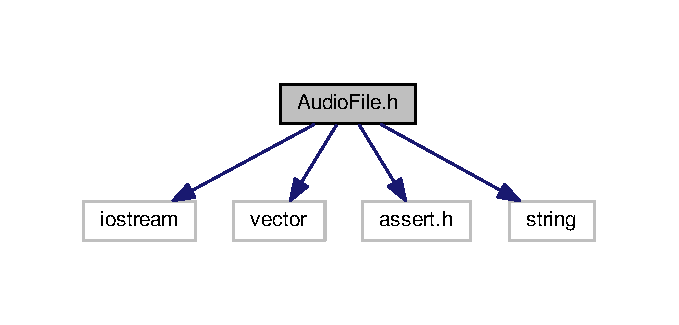
\includegraphics[width=326pt]{_audio_file_8h__incl}
\end{center}
\end{figure}
This graph shows which files directly or indirectly include this file\+:\nopagebreak
\begin{figure}[H]
\begin{center}
\leavevmode
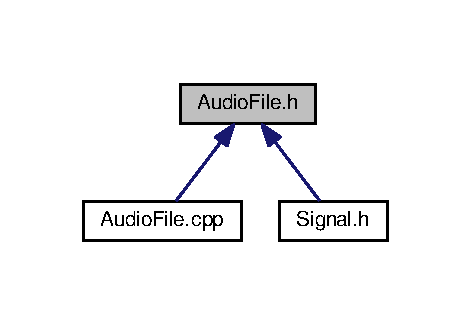
\includegraphics[width=226pt]{_audio_file_8h__dep__incl}
\end{center}
\end{figure}
\subsection*{Classes}
\begin{DoxyCompactItemize}
\item 
class \hyperlink{class_audio_file}{Audio\+File$<$ T $>$}
\end{DoxyCompactItemize}
\subsection*{Enumerations}
\begin{DoxyCompactItemize}
\item 
enum \hyperlink{_audio_file_8h_ad18559d169602e85d0ad68da6ef8593f}{Audio\+File\+Format} \{ {\bfseries Error}, 
{\bfseries Not\+Loaded}, 
{\bfseries Wave}, 
{\bfseries Aiff}
 \}
\end{DoxyCompactItemize}


\subsection{Detailed Description}
\begin{DoxyAuthor}{Author}
Adam Stark 
\end{DoxyAuthor}
\begin{DoxyCopyright}{Copyright}
Copyright (C) 2017 Adam Stark
\end{DoxyCopyright}
This file is part of the \textquotesingle{}\hyperlink{class_audio_file}{Audio\+File}\textquotesingle{} library

This program is free software\+: you can redistribute it and/or modify it under the terms of the G\+NU General Public License as published by the Free Software Foundation, either version 3 of the License, or (at your option) any later version.

This program is distributed in the hope that it will be useful, but W\+I\+T\+H\+O\+UT A\+NY W\+A\+R\+R\+A\+N\+TY; without even the implied warranty of M\+E\+R\+C\+H\+A\+N\+T\+A\+B\+I\+L\+I\+TY or F\+I\+T\+N\+E\+SS F\+OR A P\+A\+R\+T\+I\+C\+U\+L\+AR P\+U\+R\+P\+O\+SE. See the G\+NU General Public License for more details.

You should have received a copy of the G\+NU General Public License along with this program. If not, see \href{http://www.gnu.org/licenses/}{\tt http\+://www.\+gnu.\+org/licenses/}. 

\subsection{Enumeration Type Documentation}
\mbox{\Hypertarget{_audio_file_8h_ad18559d169602e85d0ad68da6ef8593f}\label{_audio_file_8h_ad18559d169602e85d0ad68da6ef8593f}} 
\index{Audio\+File.\+h@{Audio\+File.\+h}!Audio\+File\+Format@{Audio\+File\+Format}}
\index{Audio\+File\+Format@{Audio\+File\+Format}!Audio\+File.\+h@{Audio\+File.\+h}}
\subsubsection{\texorpdfstring{Audio\+File\+Format}{AudioFileFormat}}
{\footnotesize\ttfamily enum \hyperlink{_audio_file_8h_ad18559d169602e85d0ad68da6ef8593f}{Audio\+File\+Format}\hspace{0.3cm}{\ttfamily [strong]}}

The different types of audio file, plus some other types to indicate a failure to load a file, or that one hasn\textquotesingle{}t been loaded yet 
%--- End generated contents ---

% Index
\backmatter
\newpage
\phantomsection
\clearemptydoublepage
\addcontentsline{toc}{chapter}{Index}
\printindex

\end{document}
